\begin{figure}[H]
    \begin{subfigure}{0.23\linewidth}
        \centering
        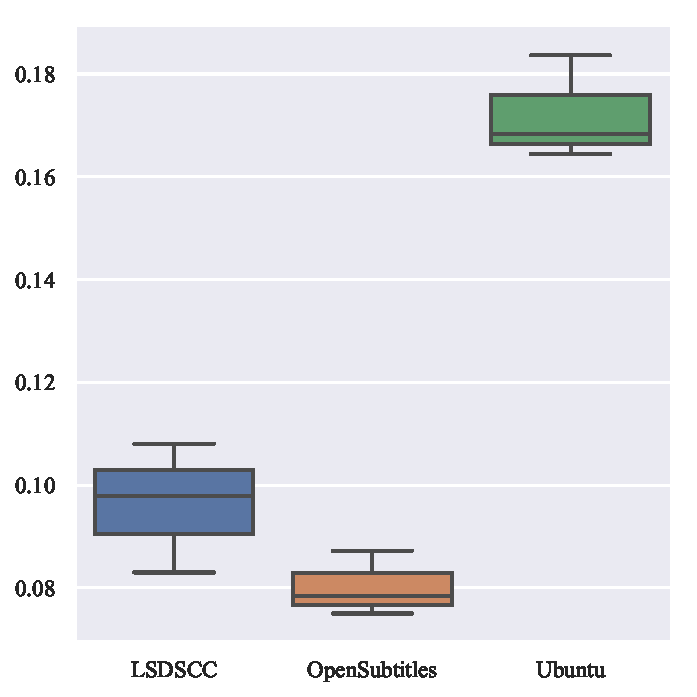
\includegraphics[width=\linewidth]{figure/boxplot/dataset/rouge_1/plot.pdf}
        \caption{ROUGE-1}
    \end{subfigure}%
    \begin{subfigure}{0.23\linewidth}
        \centering
        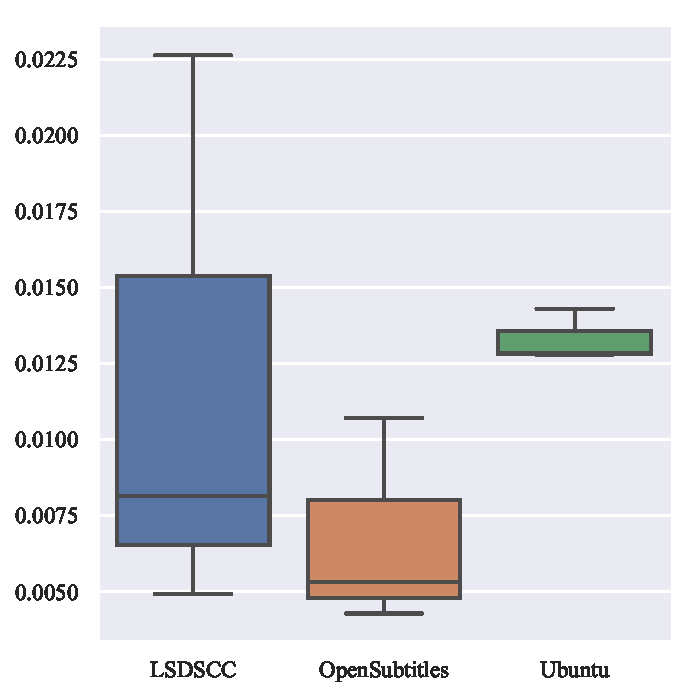
\includegraphics[width=\linewidth]{figure/boxplot/dataset/rouge_2/plot.pdf}
        \caption{ROUGE-2}
    \end{subfigure}%
    \begin{subfigure}{0.23\linewidth}
        \centering
        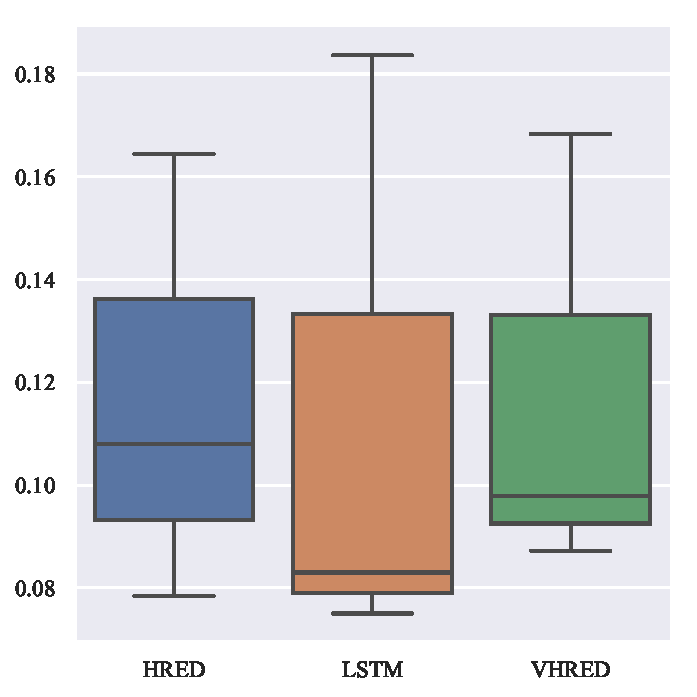
\includegraphics[width=\linewidth]{figure/boxplot/model/rouge_1/plot.pdf}
        \caption{ROUGE-1}
    \end{subfigure}%
    \begin{subfigure}{0.23\linewidth}
        \centering
        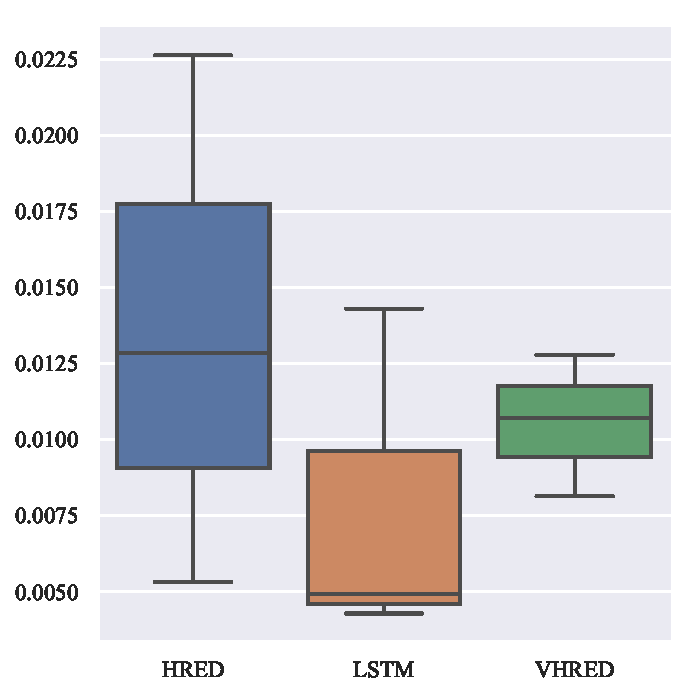
\includegraphics[width=\linewidth]{figure/boxplot/model/rouge_2/plot.pdf}
        \caption{ROUGE-2}
    \end{subfigure}
    \begin{subfigure}{0.23\linewidth}
        \centering
        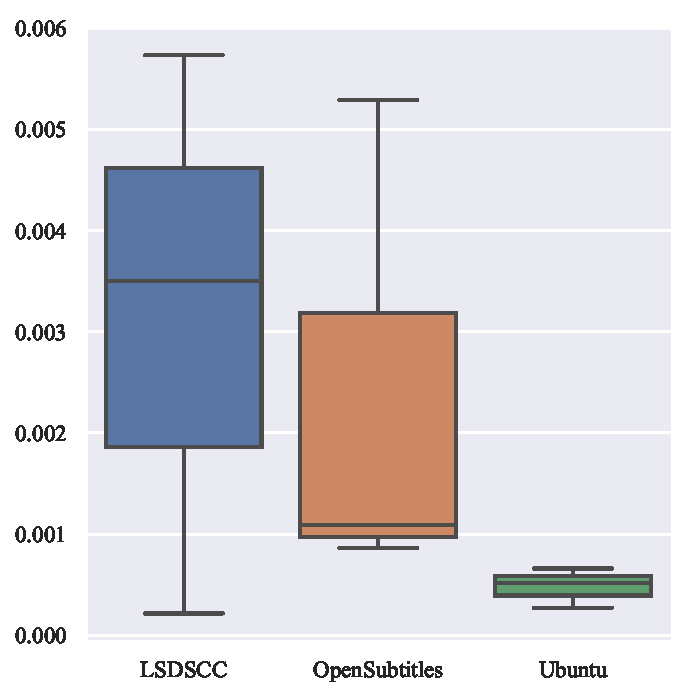
\includegraphics[width=\linewidth]{figure/boxplot/dataset/rouge_3/plot.pdf}
        \caption{ROUGE-3}
    \end{subfigure}%
    \begin{subfigure}{0.23\linewidth}
        \centering
        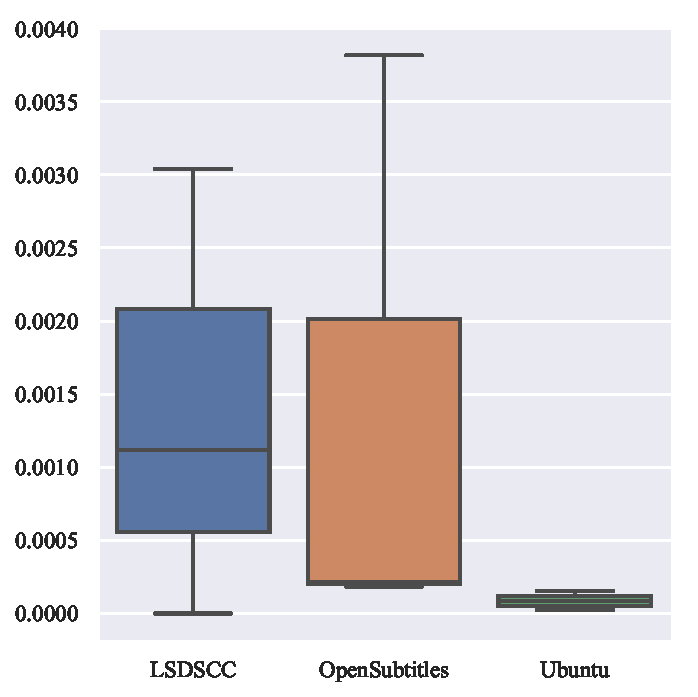
\includegraphics[width=\linewidth]{figure/boxplot/dataset/rouge_4/plot.pdf}
        \caption{ROUGE-4}
    \end{subfigure}%
    \begin{subfigure}{0.23\linewidth}
        \centering
        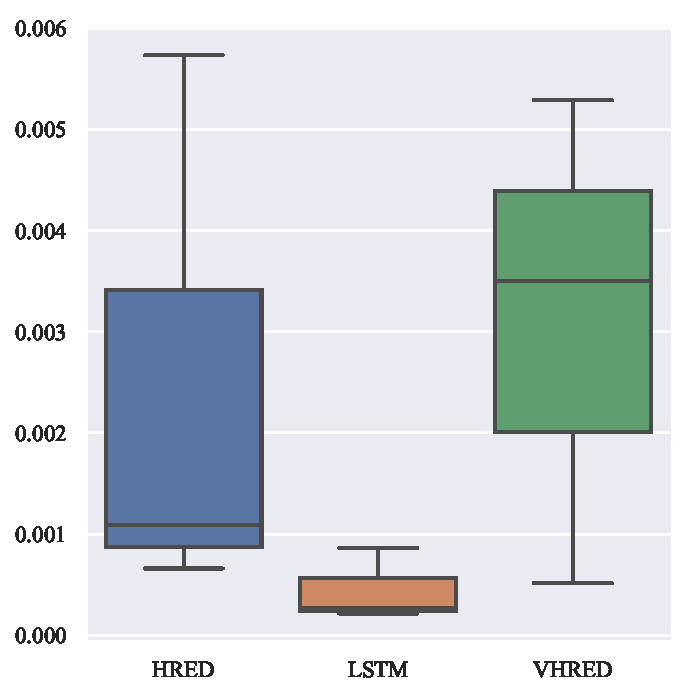
\includegraphics[width=\linewidth]{figure/boxplot/model/rouge_3/plot.pdf}
        \caption{ROUGE-3}
    \end{subfigure}%
    \begin{subfigure}{0.23\linewidth}
        \centering
        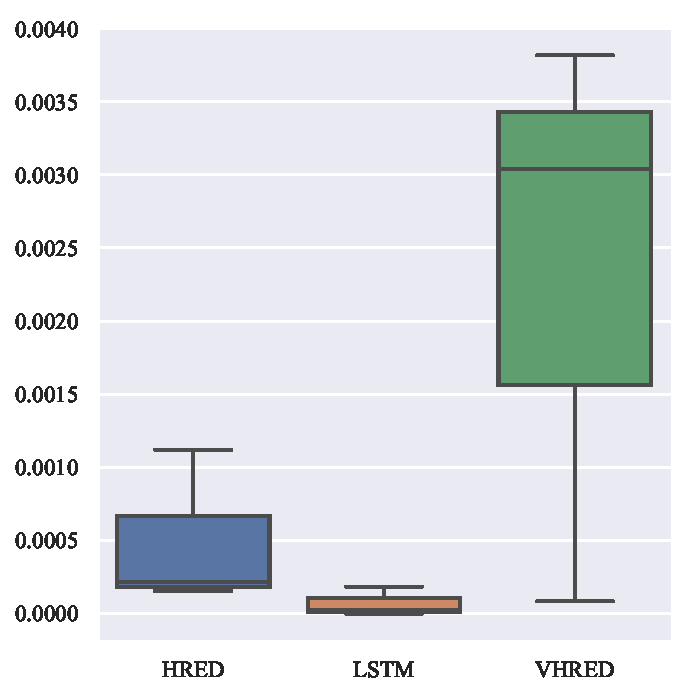
\includegraphics[width=\linewidth]{figure/boxplot/model/rouge_4/plot.pdf}
        \caption{ROUGE-4}
    \end{subfigure}
    \begin{subfigure}{0.23\linewidth}
        \centering
        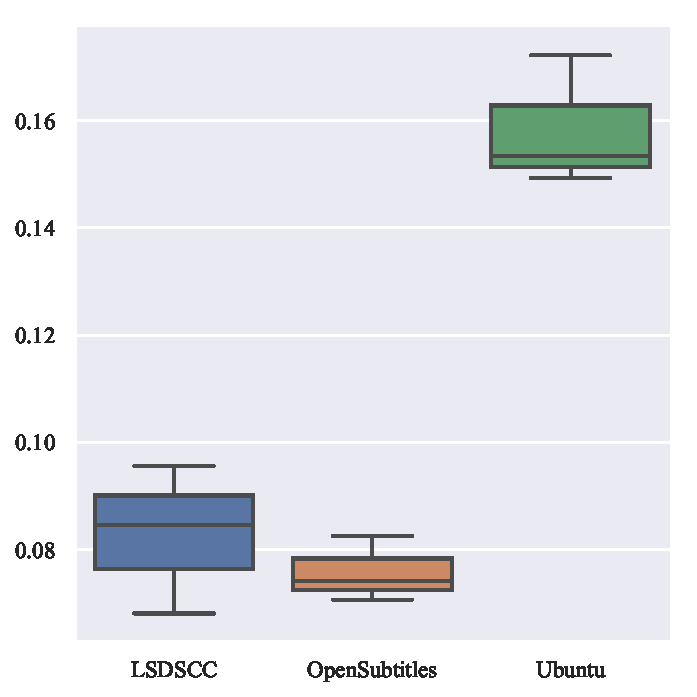
\includegraphics[width=\linewidth]{figure/boxplot/dataset/rouge_l/plot.pdf}
        \caption{ROUGE-L}
    \end{subfigure}%
    \begin{subfigure}{0.23\linewidth}
        \centering
        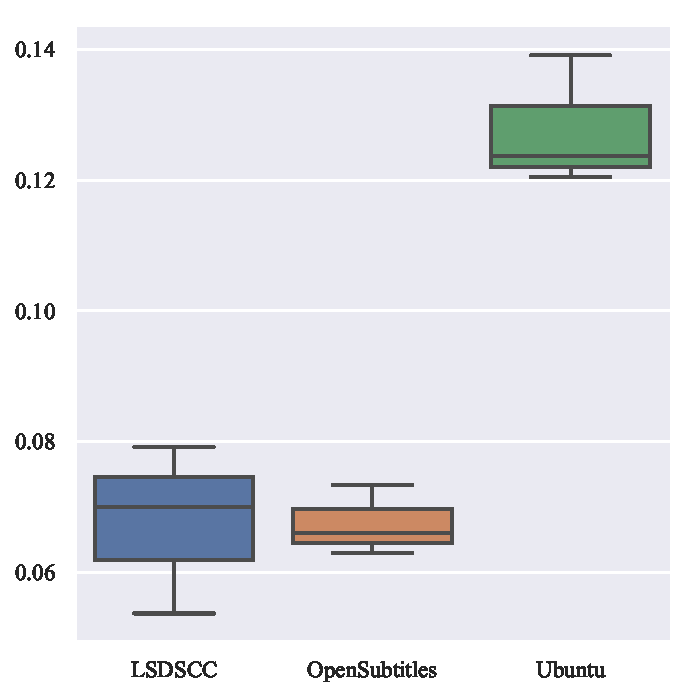
\includegraphics[width=\linewidth]{figure/boxplot/dataset/rouge_w/plot.pdf}
        \caption{ROUGE-W}
    \end{subfigure}%
    \begin{subfigure}{0.23\linewidth}
        \centering
        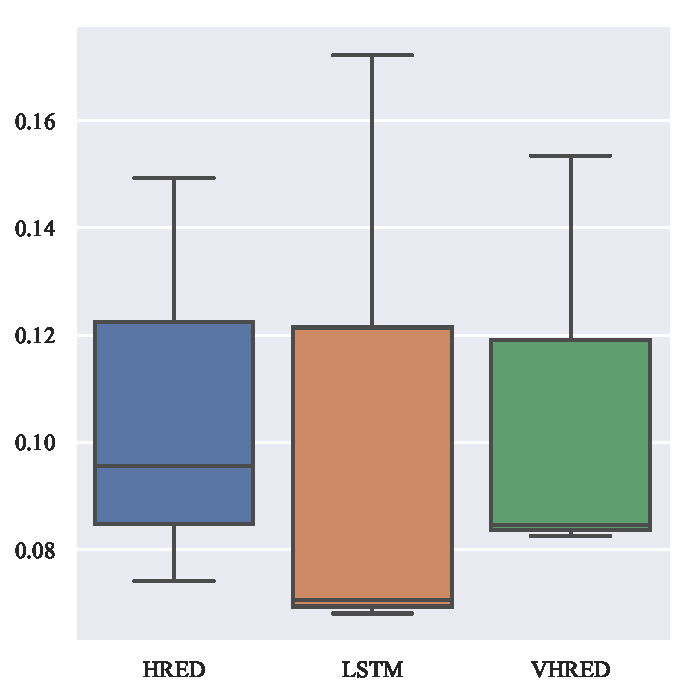
\includegraphics[width=\linewidth]{figure/boxplot/model/rouge_l/plot.pdf}
        \caption{ROUGE-L}
    \end{subfigure}%
    \begin{subfigure}{0.23\linewidth}
        \centering
        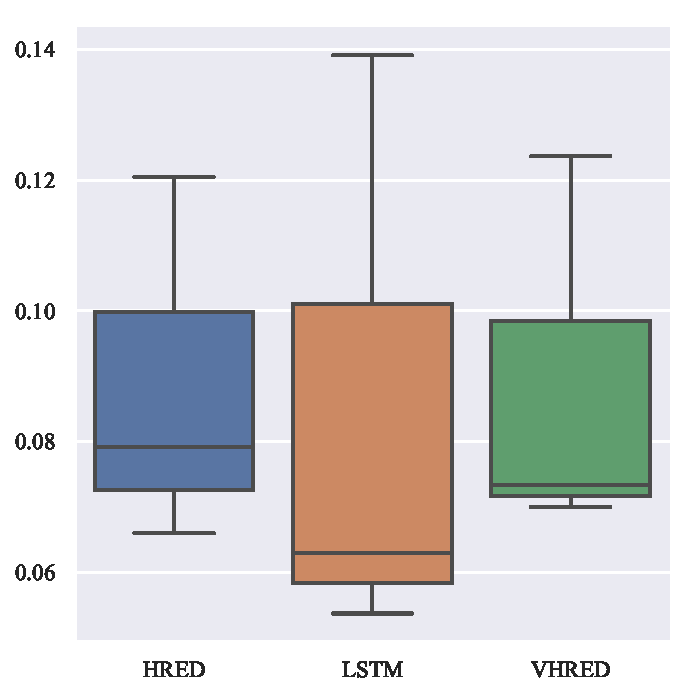
\includegraphics[width=\linewidth]{figure/boxplot/model/rouge_w/plot.pdf}
        \caption{ROUGE-W}
    \end{subfigure}
    \begin{subfigure}{0.23\linewidth}
        \centering
        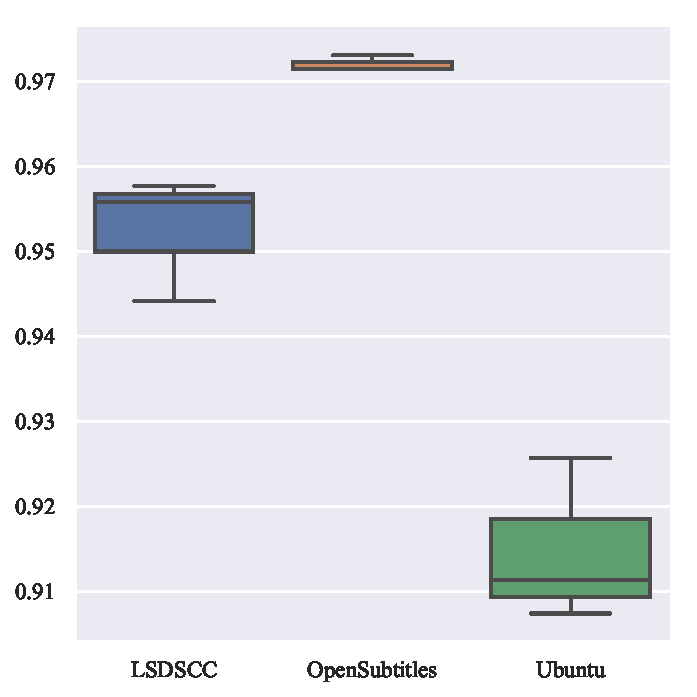
\includegraphics[width=\linewidth]{figure/boxplot/dataset/distinct_1/plot.pdf}
        \caption{Distinct-1}
    \end{subfigure}%
    \begin{subfigure}{0.23\linewidth}
        \centering
        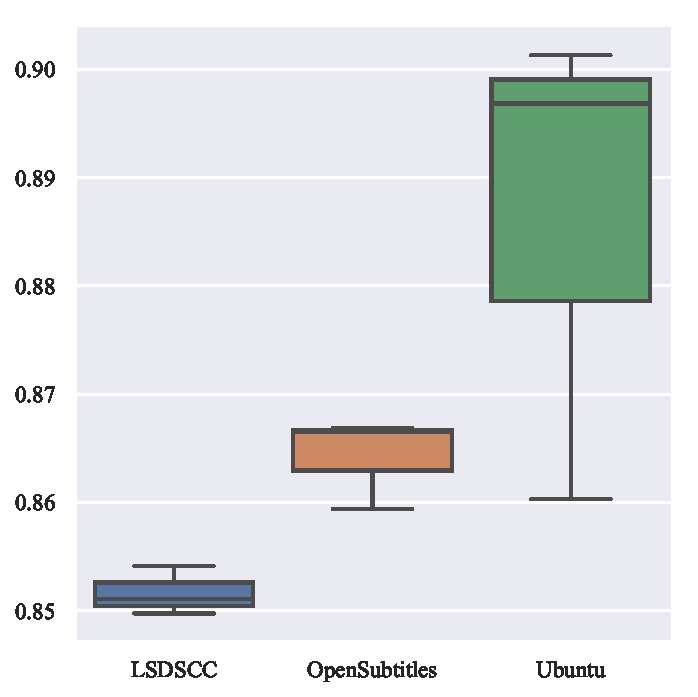
\includegraphics[width=\linewidth]{figure/boxplot/dataset/distinct_2/plot.pdf}
        \caption{Distinct-2}
    \end{subfigure}%
    \begin{subfigure}{0.23\linewidth}
        \centering
        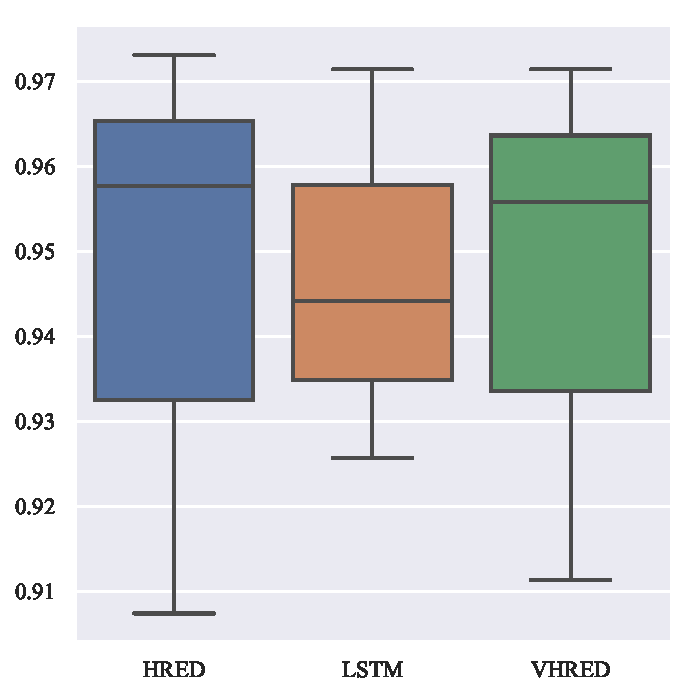
\includegraphics[width=\linewidth]{figure/boxplot/model/distinct_1/plot.pdf}
        \caption{Distinct-1}
    \end{subfigure}%
    \begin{subfigure}{0.23\linewidth}
        \centering
        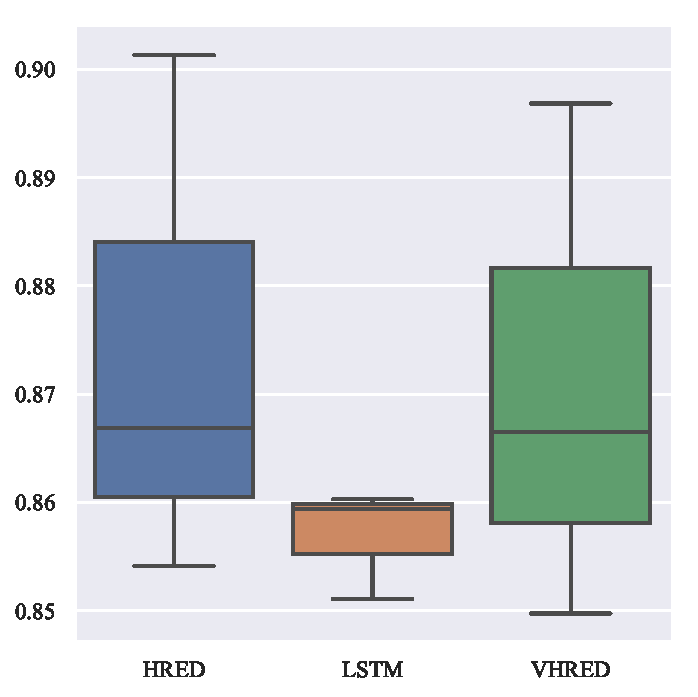
\includegraphics[width=\linewidth]{figure/boxplot/model/distinct_2/plot.pdf}
        \caption{Distinct-2}
    \end{subfigure}
    \begin{subfigure}{0.23\linewidth}
        \centering
        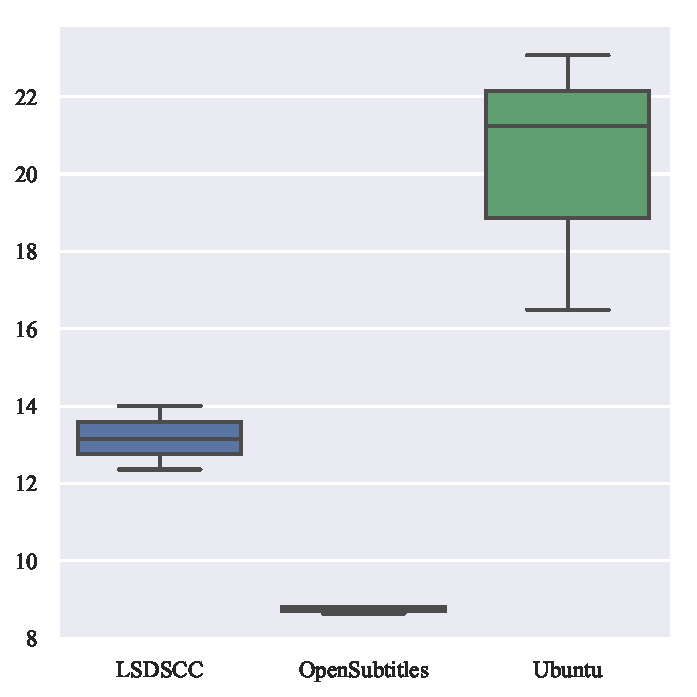
\includegraphics[width=\linewidth]{figure/boxplot/dataset/utterance_len/plot.pdf}
        \caption{\#words}
    \end{subfigure}%
    \begin{subfigure}{0.23\linewidth}
        \centering
        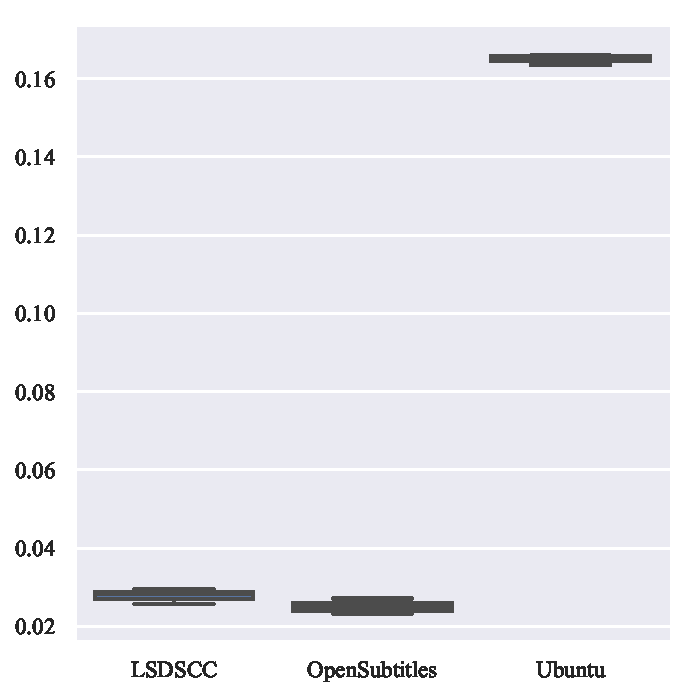
\includegraphics[width=\linewidth]{figure/boxplot/dataset/meteor/plot.pdf}
        \caption{METEOR}
    \end{subfigure}%
    \begin{subfigure}{0.23\linewidth}
        \centering
        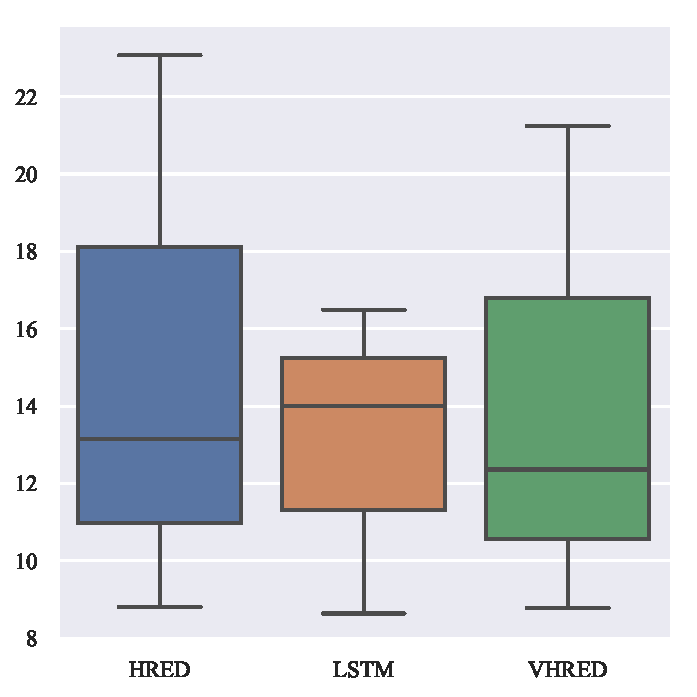
\includegraphics[width=\linewidth]{figure/boxplot/model/utterance_len/plot.pdf}
        \caption{\#words}
    \end{subfigure}%
    \begin{subfigure}{0.23\linewidth}
        \centering
        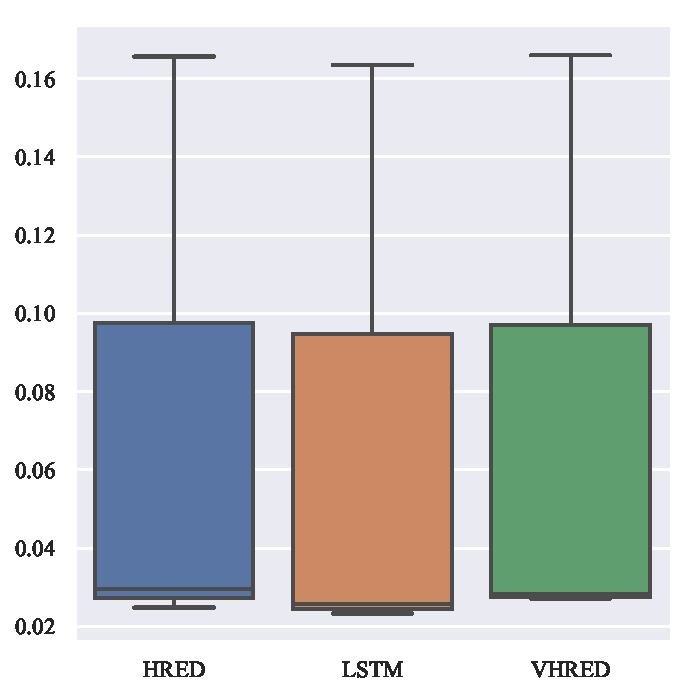
\includegraphics[width=\linewidth]{figure/boxplot/model/meteor/plot.pdf}
        \caption{METEOR}
    \end{subfigure}
    \centering
    \caption{指标在不同数据集上的分布(左)和在不同模型上的分布(右)}
\end{figure}
